\documentclass{article}

\usepackage{graphicx} % more modern
\usepackage{subfigure} 
\usepackage{amssymb}
\usepackage{amsmath}
\usepackage{amsthm}


% For citations
\usepackage{natbib}

% For algorithms
\usepackage{comment}
\usepackage{framed}
\usepackage{algorithm}
\usepackage{algorithmic}
\usepackage{amsmath}
%\usepackage{algorithmicx}
%\usepackage{algpseudocode}

\usepackage{hyperref}

\allowdisplaybreaks

\newcommand{\theHalgorithm}{\arabic{algorithm}}

\newtheorem{theorem}{Theorem}[section]
\newtheorem{lemma}[theorem]{Lemma}
\newtheorem{conjecture}[theorem]{Conjecture}
\newtheorem{proposition}[theorem]{Proposition}
\newtheorem{definition}[theorem]{Definition}
\newtheorem{corollary}[theorem]{Corollary}

%\usepackage[accepted]{icml2014}  % XXX : just set temporarly to print out authors corretly.
\usepackage{icml2014}  

\renewcommand{\algorithmicrequire}{\textbf{Input:}}
\renewcommand{\algorithmicensure}{\textbf{Output:}}

\begin{document} 

\icmltitle{Exploiting Linear Structure Within Convolutional Networks
  for Efficient Evaluation}

\icmlauthor{Emily Denton}{denton@cs.nyu.edu}
\icmlauthor{Wojciech Zaremba}{zaremba@cs.nyu.edu}
\icmlauthor{Joan Bruna}{bruna@cs.nyu.edu}
\icmlauthor{Rob Fergus}{fergus@cs.nyu.edu}

\icmlkeywords{machine learning, deep learning, speeding up forward pass, redundancies in neural networks}


\begin{abstract}
We present techniques for speeding up the test-time evaluation of large convolutional networks, designed for object recognition tasks. These models deliver impressive accuracy but each image evaluation requires millions of floating point operations, making their deployment on smartphones and Internet-scale clusters problematic. The computation is dominated by the convolution operations in the lower layers of the model. We exploit the linear structure present within the 
convolutional filters to derive approximatations that significantly reduce the required computation. Using large state-of-the-art models, we demonstrate speedups by a factor of $2-4$x, while keeping the accuracy within $1\%$ of the original model. 
\end{abstract}

\section{Introduction}

Large neural networks have recently demonstrated impressive
performance on a range of speech and vision tasks. However the size of
these models can make their deployment at test time problematic. For
example, mobile computing platforms are limited in their CPU speed,
memory and battery life. At the other end of the spectrum,
Internet-scale deployment of these models requires thousands of
servers to process the 100's of millions of images per day. The
electrical and cooling costs of these servers required is significant.

Training large neural networks (NN) can take weeks, or even
months. This hinders research and consequently there have been
extensive efforts devoted to speeding up training procedure.  However,
there are relatively few efforts are improving the {\em test-time}
performance of the models. 

In this paper we focus on speeding up the
evaluation of {\em trained} networks, without compromising
performance. We consider convolutional neural networks used for
computer vision tasks, since they are large and widely used in
commercial applications. Within these models, most of the time ($\sim90\%$) is spent in the
convolution operations in the lower layers of the model. The remaining
operations: pooling, contrast normalization and the upper
fully-connected layers collectively take up the remaning $10\%$.

We present two novel methods for speeding up the convolution
operations. One involves projecting the input image into a set of 1-D
color sub-spaces. This allows the filters in the first of layer of the
model to be monochromatic (i.e. reducing the color channels from three
to one), thereby saving a factor of 3 in computation. The second
approach, applied to subsequent convolution layers, involves
clustering the filters into a set of low-dimensional linear
sub-spaces, each of which is represented by a set of tensor
outer-products. Collectively, our techniques speed up execution by
factor of $2-4$ while keeping prediction accuracy within $1\%$ of the
original model. These gains allow the use of larger, higher
performance models than would otherwise be practical.


% resource-wise from perspective of companies executing neural networks on internet-scale
% data (e.g. annotating images), this is not the main cost. Major cost is in the
% final stage, where network is evaluated on the target data, which is present in quantities of billions.
% We focus here on speeding up evaluation of \emph{trained} NN, which directly
% maps to the cost of executing NN on internet-scale data.

% % XXX: Maybe we will speak also about real time application.


% We focus in this work on convolutional neural networks used for computer vision tasks. Most of
% computation time during evaluation is spend on convolutional layers i.e. $\sim90\% - 95\%$, while it takes only
% the small fraction of time $\sim 5\%-10\%$ to evaluate rest of layers (pooling, local contrast normalization,
% fully connected). It is worth to note, that most of learnable parameters are kept in fully connected layers $\sim 90\% - 95\%$
% , and convolutional layers constitutes of very small fraction of parameters $\sim 5\% - 10\%$.


% We achieve forward pass speed up by constructing approximations to the convolutional layer kernel. Convolutional kernel
% is a $4$-dimensional tensor, with two spacial dimensions, and two feature maps-to-feature maps dimensions. Kernel of trained
% network has a lot of redundancies in parameters, which we exploit to speed up forward pass, while mildly training off
% prediction accuracy (approximated kernels give prediction within $\sim 1\%$ of the original prediction).


\section{Related Work}
%There have been extensive research devoted speeding up forward pass of neural network. 
%There are few different pathways, how the speed up can be achieved. 


\cite{vanhoucke2011improving} explored the
properties of CPUs to speed up execution.  They present many solutions
specific to Intel and AMD CPUs, however some of their techniques are
general enough to be used for any type of processor.  They describe
how to align memory, and use SIMD operations (vectorized operations on
CPU) to boost the efficiency of matrix multiplication.  Additionally, they
propose the linear quantization of the network weights and input. This
involves representing weights as 8-bit integers (range
$[-1287 128]$), rather than 32-bit floats. This approximation is
similar in spirit to our approach, but differs in that it is applied
to each weight element independently. By contrast, our approximation approach models
the structure within each filter. Potentially, the two approaches
could be used in conjunction. 

% combinIt can also potentially be to 
% approximates the ion, it does so based on the structure of the weights.  each which
% replaces kernel $W$ with few other operations, which give result
% approximately equal to convolution with $W$. Moreover, linear
% quantization can be used in conjunction with methods presented in this
% paper.



The most expensive operations in convolutional networks are the
convolutions in the first few layers. The complexity of this operation
is linear in the area of the receptive field of the filters, which is
relatively large for these layers.  However, \cite{mathieu2013fast} have shown that convolution can be
efficiently computed in Fourier domain, where it becomes element-wise
multiplication (and there is no cost associated with size of receptive
field). They report a forward-pass speed up of around $10x$ (depending on
the kernel size, number of features etc.).  Importantly, this method can
be used jointly with most of techniques presented in this paper.

The use of low-rank approximations in our approach is inspired by work
of \cite{denil2013predicting} who demonstrate the redundancies in neural
network parameters. They show that the weights within a layer can be
accurately predicted from a small (e.g. $\sim 5\%$) subset of them. This
indicates that neural networks are heavily over-parametrized.  All the
methods presented here focus on exploiting the linear structure of this
over-parametrization.

\section{Framework}
We utilize in our studies models trained on Imagenet 2012 dataset. One is developed
by Alex Krizhevsky\cite{krizhevsky2012imagenet}, and other by Matthew Zeiler \cite{zeiler2013visualizing}.
We refer to them respectively as AlexNet, and MattNet. We evaluate our networks on Macbook pro with i7 Intel processor, and
all our evaluation code is in implemented in C++ using eigen3 library \cite{eigenweb}.


\section{Low Rank Approximations}
In this section, we give theoretical background on low rank approximations. First, we discuss simplest setting, which is
for matrices (two dimensional tensors). We then consider the approximation of 4-dimensional tensors of convolution weights.


\subsection{Matrix Low Rank Approximation}
Let $X \in \mathbb{R}^{n \times m}$ denote the input to a fully connected layer of a neural network and let $W \in \mathbb{R}^{m \times k}$ denote the weight matrix for the layer. Matrix multiplication,  the main operation for fully connected layers, costs $O(nmk)$. However, $W$ is likely to have a low-rank structure and thus have several eigenvalues close to zero. These dimensions can be interpreted as noise, and thus can be eliminated without harming the accuracy of the network. We now show how to exploit this low-rank structure and to $XW$ much faster than $O(nmk)$. 


Every matrix $W \in \mathbb{R}^{m \times k}$ can be expressed using singular value decomposition:
\begin{equation*}
	W = USV^{\top}\text{, where }U \in \mathbb{R}^{m \times m}, S \in \mathbb{R}^{m \times k}, V \in \mathbb{R}^{k \times k}
\end{equation*}
$S$ is has eigenvalues on the diagonal, and zeros elsewhere. $W$ can be approximated by choosing the $t$ largest 
eigenvalues from $S$. We can write the approximation as
\begin{equation*}
	\hat{W} = \tilde{U}\tilde{S}\tilde{V}^{\top}\text{, where }\tilde{U} \in \mathbb{R}^{m \times t}, \tilde{S} \in \mathbb{R}^{t \times t}, \tilde{V} \in \mathbb{R}^{t \times k}
\end{equation*}

Now the computation $X\tilde{W}$ can be done in $O(nmt + nt^2 + ntk)$, which, for sufficiently small $t$ can be significantly smaller than $O(nmk)$. 

\subsection{Tensor Low Rank Approximations}

In typical object recognition architectures, the convolutional layer weights at the end of training exhibit strong redundancy and regularity across all dimensions. A particularly simple way to exploit such regularity is to 
linearly compress the tensors, which amounts to finding low-rank approximations.

Convolution weights can be described as a $4$-dimensional tensor. Let $W \in \mathbb{R}^{C \times X \times Y \times F}$ 
denote such a weight tensor. $C$ is the number of number of input channels, $X$ and $Y$ are the special dimensions of the kernel, and $F$ is the target number of feature maps.
Let $I \in \mathbb{R}^{C \times N \times M}$ denote an input signal where $C$ is the number of input maps, and $N$ and $M$ are the spatial dimensions of the maps.
The computation performed by a generic convolutional layer is defined as
\begin{align*}
\label{convlayereq}
&I \ast W (f,x,y) = \\
&\sum_{c=1}^C \sum_{x'=1}^{X} \sum_{y'=1}^{Y} I(c,x+x',y+y') W(c,x',y',f)
\end{align*}

We would like to approximate $W$ with a low rank tensor that has a particular structure that allows for a more efficient computation of the convolution. The approximations will be more efficient in two senses: both the number of floating point operations required to compute the convolution output and the number of parameters that need to be stored will be dramatically reduced. 

A standard first convolutional layer will receives three color channels, typically in RGB or YUV space, as input whereas later hidden layers typically receive a much larger number of feature maps that have resulted from computations performed in previous layers. As a result, the first layer weights often have a markedly different structure than the weights in later convolutional layers. We have found that different approximation techniques are well suited to the different layers which we now describe. The first approach, which we call the monochromatic filter approximation can be applied to the weights in the first convolutional layer. The second approach, which we call the bi-clustering approximation,  can be applied to later convolutional layers where the number of input and output maps is large. 

\subsection{Monochromatic filters}
Let $W \in \mathbb{R}^{C \times X \times Y \times F}$ denote the first convolutional layer weights of a trained network. The number of input channels, $C$, is 3 and each channel corresponds to a different color component (either RGB or YUV). We have found that the color components of weights from a trained convolutional neural network have low dimensional structure. In particular, the weights can be well approximated by projecting the color dimension down into a 1D subspace. Figure ?? shows the original first layer convolutional weights of a trained network and the weights after the color dimension has been projected into 1D lines. 

The approximation is computed as follows. First, for every output feature, $f$, we consider consider the matrix $W_f \in \mathbb{R}^{C \times XY }$, where the spatial dimensions have been combined, and find the singular value decomposition, 
\begin{equation*}
	W_f = U_f S_f V_f^{\top}
\end{equation*}
where $U_f \in \mathbb{R}^{C \times C}, S_f \in \mathbb{R}^{C \times XY}, V_f \in \mathbb{R}^{XY \times XY}$. We then take the rank-1 approximation to $W_f$ 
\begin{equation*}
	\tilde{W}_f = \tilde{U}_f \tilde{S}_f \tilde{V}_f^{\top}
\end{equation*}
where $\tilde{U}_f \in \mathbb{R}^{C \times 1}, \tilde{S}_f \in \mathbb{R}, \tilde{V}_f \in \mathbb{R}^{1 \times XY}$.

This approximation corresponds to shifting from $C$ color channels to 1 color channel for each output feature. We can further exploit the regularity in the weights by sharing the color component basis between different output features. We do this by clustering the $F$ left singular vectors,  $\tilde{U}_f$, of each output feature $f$ into $C'$ different equal sized clusters, where $C'$ is much smaller than $F$. Then, for each of the $\frac{F}{C'}$ output feature, $f$, that is assigned to cluster $c$, we can approximate $W_f$ with
\begin{equation*}
	\tilde{W}_f = U_c \tilde{S}_f \tilde{V}_f^{\top}
\end{equation*}
where $U_c \in \mathbb{R}^{C \times 1}$ is the cluster center for cluster $c$ and $\tilde{S}_f$ and $\tilde{V}_f$ as as before. 

This low-rank approximation allows for a more efficient computation of the convolutional layer output. By decomposing the approximated weights into two tensors. Let $W_C \in \mathbb{R}^{C' \times C}$ denote the color transform matrix where the rows of $W_c$ are the cluster centers $U_c^{\top}$. Let $W_{mono} \in \mathbb{R}^{X \times Y \times F}$ denote the monochromatic weight tensor containing $ \tilde{S}_f \tilde{V}_f^{\top}$ for each of the $F$ output features. Given this decomposition, we can compute the output of the convolutional layer by first transforming the input signal, $I \in \mathbb{R}^{C \times N \times M}$ into a different basis using the color transform matrix: $\tilde{I} = W_c$. 


\subsection{Bi-clustering of hidden layer weights}








\subsection{Monochromatic filters}
Let $W \in \mathbb{R}^{C \times X \times Y \times F}$ denote the first convolutional layer weights of a trained network. The number of input channels, $C$, is 3 and each channel corresponds to a different color component (either RGB or YUV). We found that the color components of weights from a trained convolutional neural network have low dimensional structure. In particular, the weights can be well approximated by projecting the color dimension down into a 1D subspace. Figure ?? shows the original first layer convolutional weights of a trained network and the weights after the color dimension has been projected into 1D lines. 

The approximation for this layer exploits this low dimensional structure and is computed as follows. First, for every output feature, $f$, we consider consider the matrix $W_f \in \mathbb{R}^{C \times XY }$, where the spatial dimensions of the filter corresponding to the output feature have been combined, and find the singular value decomposition, 
\begin{equation*}
	W_f = U_f S_f V_f^{\top}
\end{equation*}
where $U_f \in \mathbb{R}^{C \times C}, S_f \in \mathbb{R}^{C \times XY}, V_f \in \mathbb{R}^{XY \times XY}$. We then take the rank 1 approximation to $W_f$ 
\begin{equation*}
	\tilde{W}_f = \tilde{U}_f \tilde{S}_f \tilde{V}_f^{\top}
\end{equation*}
where $\tilde{U}_f \in \mathbb{R}^{C \times 1}, \tilde{S}_f \in \mathbb{R}, \tilde{V}_f \in \mathbb{R}^{1 \times XY}$.

This approximation corresponds to shifting from $C$ color channels to 1 color channel for each output feature. We can further exploit the regularity in the weights by sharing the color component basis between different output features. We do this by clustering the $F$ left singular vectors,  $\tilde{U}_f$, of each output feature $f$ into $C'$ equal sized clusters, where $C'$ is much smaller than $F$. Then, for each of the $\frac{F}{C'}$ output features, $f$, that is assigned to cluster $c$, we can approximate $W_f$ with
\begin{equation*}
	\tilde{W}_f = U_c \tilde{S}_f \tilde{V}_f^{\top}
\end{equation*}
where $U_c \in \mathbb{R}^{C \times 1}$ is the cluster center for cluster $c$ and $\tilde{S}_f$ and $\tilde{V}_f$ as as before. 

By decomposing the approximated weights into two tensors, this low-rank approximation allows for a more efficient computation of the convolutional layer output. Let $W_C \in \mathbb{R}^{C' \times C}$ denote the color transform matrix where the rows of $W_c$ are the cluster centers $U_c^{\top}$. Let $W_{mono} \in \mathbb{R}^{X \times Y \times F}$ denote the monochromatic weight tensor containing $ \tilde{S}_f \tilde{V}_f^{\top}$ for each of the $F$ output features. Given this decomposition, we can compute the output of the convolutional layer by first transforming the input signal, $I \in \mathbb{R}^{C \times N \times M}$ into a different basis using the color transform matrix: 
\begin{equation*}
	\tilde{I} = W_c \otimes I
\end{equation*}
where $\tilde{I} \in \mathbb{R}^{C' \times N \times M}$. After the color transformation, each of the $f$ filters in $W_{mono}$ is monochromatic in the sense that it only acts upon one of the $C'$ color channels. The fact that we can do this approximation without hurting performance indicates that the structure inherent in the learned first convolutional layer weights of a network make it such that, in a new basis, the connections between input and output maps become sparse. To be specific, target value, $\tilde{T}$, of the approximated convolutional layer for a particular output feature $f$, and spatial location $(x, y)$ is
\begin{align*}
	\tilde{T}(f, x, y) &= \sum_{x' = 1}^{X} \sum_{y' = 1}^{Y} \Big(\sum_{c = 1}^{C} I(c, x + x', y + y') W_c(c', c) \Big) \\
			&\hspace{3mm} \times (c, x + x', y + y') W(x', y', f) \\
			&= \sum_{x' = 1}^{X} \sum_{y' = 1}^{Y} \tilde{I}(c', x + x', y + y') W(x', y', f)
\end{align*} 
where $c' \in [1, ..., C']$ is the cluster feature $f$ is assigned to. If the color transformation is computed once at the outset, then the number of operations performed is significantly reduced.  

\subsubsection{Complexity analysis}
By using the monochromatic filter approximation to the first layer convolutional weights, the target output can be computed with significantly fewer operations. The number of operations that will be required is a function the number of color components, $C'$, that are used in the approximation. Table \ref{monochromatic_ops} gives the number of operations required in the original and approximated cases as a function of $C'$. 

\begin{table}[h]
\tiny
\parbox{\linewidth}{
\centering
\begin{tabular}{cc}
\hline
Original & Approximated \\
\hline
$C X Y F N M \Delta^{-2}$  & $	 C' C^2 N M + X Y F N M \Delta^{-2}$\\
\hline
\end{tabular}
\caption{Number of operations required to compute target output of first convolutional layer with original weights vs. monochromatic approximation, where $\Delta$ is the stride of the filter.}
\label{monochromatic_ops}
}
\end{table}

Figure \ref{monochromatic_ops_pic} shows the relative reduction in operations for varying values of $C'$.

\begin{figure}[t]
\mbox{
  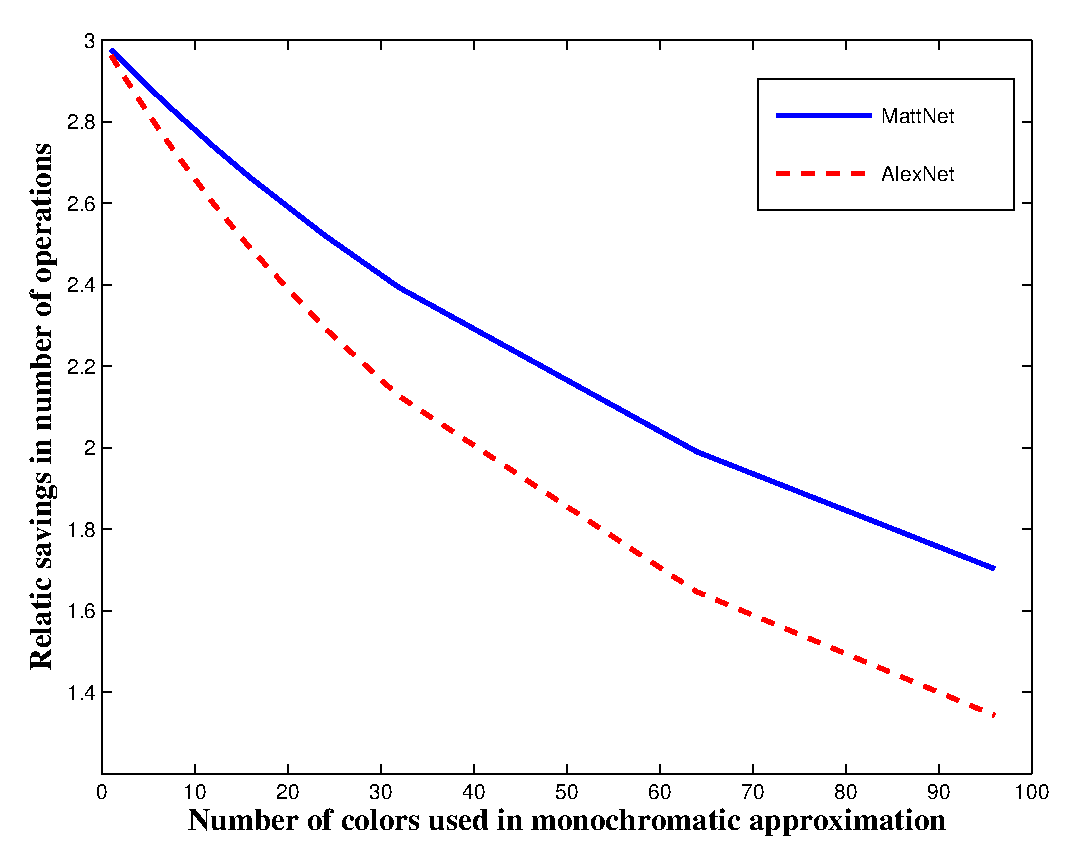
\includegraphics[width=\linewidth]{img/monochromatic_numcolors_vs_numops.eps} 
}
\label{monochromatic_ops_pic}
\caption{Relative decrease in number of operations required to compute output of first convolutional layer for various monochromatic operations applied to MattNet (blue) and AlexNet (red).}
\end{figure}

\subsubsection{Empirical performance}
There is an obvious tradeoff between increased efficiency and decreased accuracy of the network as we approximate the filters with varying values of $C'$. In our experiments we only used approximations that did not increase the error of the network. However, it is insightful to see how test error varies with the number of color components used. Figure ?? illustrates the tradeoff.


\subsection{Bi-clustering of hidden layer weights}
Let $W \in \mathbb{R}^{C \times X \times Y \times F}$ denote the weights of a second or later convolutional layer. Similar to the first convolutional layer approximation, we rely on the low dimensional linear structure of learned weights in a trained convolutional network to find an efficient approximation. We decompose $W$ by considering a partition of the input features into $G$ equal sized clusters and a partition of the output features into $H$ equal sized clusters. For a given input cluster, $g$, and output cluster, $h$, we approximate the weights corresponding to the input and output features in those clusters, $W_{g,h} \in \mathbb{R}^{\frac{C}{G} \times X \times Y \times \frac{F}{H}}$, with a rank K tensor, $\tilde{W}_{g,h}$.  

We cluster the input features by concatenating the spatial and output feature dimensions of $W$ and clustering the resulting $C$ vectors in $\mathbb{R}^{XYF}$. This clustering can be done using k-means or a more sophisticated subspace clustering algorthm. In our experiments we found that often k-means was sufficient. We clustered the output features in an analogous manner and completely independently of the input clustering. 

Any 3D tensor, $M \in \mathbb{R}^{n \times m \times k}$, can be approximated by a decomposition that minimizes 
\begin{equation*}
	\|  \|
\end{equation*} 


\subsubsection{Complexity analysis}

\subsubsection{Empirical performance}



\section{Experiments}

We are going to present results on test time performance of approximation with monochromatic filters, and bi-clustering. Moreover,
we additionally support our approximations with visualizations. Major contribution is in lowered evaluation time, while kept prediction performance.
Table \ref{evaluation_time} gives us reference on prediction time for network without approximations.

\begin{table}[t]
\tiny
\parbox{.99\linewidth}{
\centering
\begin{tabular}{rrrrr}
\hline
& Evaluation & & Evaluation &  \\
Layer & Time & Fraction & Time per img. & Fraction \\
& (bs = 1) & (bs = 1) & (bs = 128) & (bs = 128) \\
\hline
Conv1 & & & & \\
MaxPool & & & & \\
LRNormal & & & & \\
Conv2 & & & & \\
MaxPool & & & & \\
LRNormal & & & & \\
Conv3 & & & & \\
MaxPool & & & & \\
Conv4 & & & & \\
Conv5 & & & & \\
MaxPool & & & & \\
FC & & & & \\
FC & & & & \\
FC & & & & \\
Softmax & & & & \\
\hline 
Total & & & & \\
\hline
\end{tabular}
\vspace{5mm}
}
\parbox{.99\linewidth}{
\centering
\begin{tabular}{rrrrr}
\hline
& Evaluation & & Evaluation &  \\
Layer & Time & Fraction & Time per img. & Fraction \\
& (bs = 1) & (bs = 1) & (bs = 128) & (bs = 128) \\
\hline
Conv1 & & & & \\
MaxPool & & & & \\
LRNormal & & & & \\
Conv2 & & & & \\
MaxPool & & & & \\
LRNormal & & & & \\
Conv3 & & & & \\
MaxPool & & & & \\
Conv4 & & & & \\
Conv5 & & & & \\
MaxPool & & & & \\
FC & & & & \\
FC & & & & \\
FC & & & & \\
Softmax & & & & \\
\hline 
Total & & & & \\
\hline
\end{tabular}
}
\caption{Evaluation time (in ms) per layer on CPU for (top) AlexNet, (bottom) MattNet. We consider real time application setting (batch size aka bs of 1), and
mass scale annotation (batch size of 128). Results averaged over 8 trials.}
\label{evaluation_time}
\end{table}



\subsection{Monochromatic Filters}
Monochromatic approximation can work well only if color components span few one dimensional subspaces. 
Figure \ref{components}, \ref{components} show that it is indeed case for both AlexNet, as
well as MattNet. In case of AlexNet, we colored with a different colors every feature map, so one dimensional structure
is clearly depicted. For MattNet, we found further low-dimensional structure. All the colors seems to lay close
to two planes. Visualization gives different color to color components laying on every plane. Moreover,
colors span one dimensional subspaces within planes. We further confirmed that monochromatic approximations
are faithful. 

Figures \ref{denoising} and \ref{denoising} shows first layer filters after approximating them 
with monochromatic filters. This corresponds to the projection on one out of ''number of clusters`` 1-dim plane (line).
One can notice that often approximated filters look cleaner than original one.


\begin{figure}[t]
\mbox{
  \subfigure{
      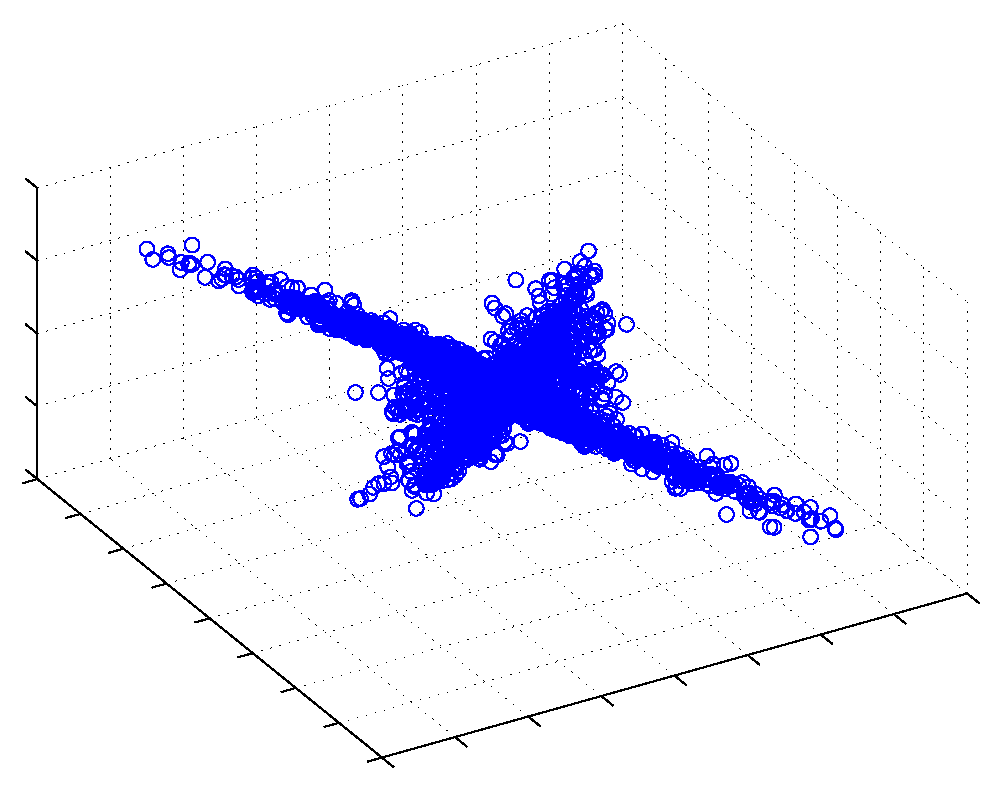
\includegraphics[width=0.45\linewidth]{img/color_components_alex_3d.eps}
  }\quad
\subfigure{
  \includegraphics[width=0.45\linewidth]{img/color_components_matthew_3d.eps} 
  }
}
\label{components}
\caption{Visualization of color components for (left) AlexNet and (right) MattNet.}
\end{figure}


\begin{figure}[t]
\mbox{
  \subfigure{
      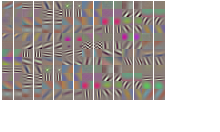
\includegraphics[width=0.45\linewidth]{img/denoising_alex.png}
  }\quad
\subfigure{
  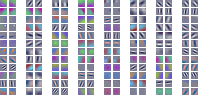
\includegraphics[width=0.45\linewidth]{img/denoising_matthew.png} 
  }
}
\label{denoising}
\caption{Left column depicts original filters, while the right one approximated one with 12 clusters for (left) AlexNet and (right) MattNet (good to look in color). }
\end{figure}


\subsection{Bi-clustering}



\section{Discussion}


\nocite{*}
\bibliography{bibliography}
\bibliographystyle{icml2014}


\end{document}






